\section{柴油机的工作原理}\label{sec:6-2}

\begin{wrapfigure}[14]{r}{6.5cm}
    \centering
    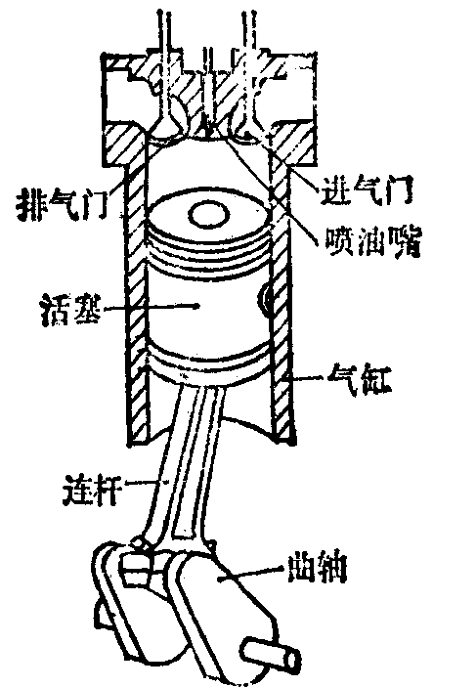
\includegraphics[width=5cm]{../pic/czwl2-ch6-2}
    \caption{柴油机}\label{fig:6-2}
\end{wrapfigure}

柴油机是用柴油作燃料的内燃机。柴油机的构造跟汽油机相似,
主要不同的是柴油机的气缸顶部有一个喷油嘴,没有火花塞(图 \ref{fig:6-2})。
柴油机的每一工作循环也是由吸气、压缩、做功和排气四个冲程组成的。
但由于使用的燃料不同,柴油机和汽油机的工作过程也有所不同。

在吸气冲程,汽油机吸入气缸里的是汽油和空气的混合物,柴油机吸入气缸里的只是空气。

\begin{enhancedline}
在压缩冲程,汽油机只把燃料混合物的体积压缩到吸气冲程末的 $\dfrac{1}{6}$ ~ $\dfrac{1}{9}$。
如果压缩得更多,在压缩过程的中途,燃料混合物就因温度升高超过燃点而燃烧,汽油机将无法正常工作。
柴油机可以把空气的体积压缩到吸气冲程末的 $\dfrac{1}{16}$ ~ $\dfrac{1}{22}$,
压强达到 35 ~ 45 千克力/$\pflm$,温度升高到 500 ~ 700 ℃ ,比汽油机里燃料混合物的压强和温度都高。
\end{enhancedline}

在做功冲程,汽油机是用火花塞点火使燃料燃烧的(这种点火方式叫做点燃式)。
柴油机是在压缩冲程末,由喷油嘴向气缸内喷射雾状柴油,
雾状柴油遇到远远超过它的燃点的热空气立即燃烧(这种点火方式叫做压燃式)。
燃气的温度达到 1700 ~ 2000 ℃ ,压强达到 50 ~ 100 千克力/$\pflm$。
在柴油机里,推动活塞做功的燃气的压强比汽油机里的高,燃气做的功较多,所以效率较高。

在排气冲程,柴油机和汽油机一样,将废气排出气缸。

柴油比汽油便宜,所以柴油机比汽油机经济,但是比较笨重,主要应用在拖拉机、坦克、轮船、内燃机车、载重汽车上。
在没有电源的地方,常用它带动水泵和各种农业加工机械工作,或带动发电机发电。

